%----------------------------------------------------------------------------------------
%	PAQUETES
%----------------------------------------------------------------------------------------

\documentclass[11pt,spanish]{article} % Default font size is 12pt, it can be changed here

\usepackage{amsmath}%
\usepackage{MnSymbol}%
\usepackage{wasysym}%

\usepackage[margin=1.25in]{geometry} % Required to change the page size to A4
\geometry{a4paper} % Set the page size to be A4 as opposed to the default US Letter

\usepackage{eurosym}

\usepackage{graphicx} % Required for including pictures

\usepackage{caption}
\captionsetup[table]{position=bottom}

\usepackage{float} % Allows putting an [H] in \begin{figure} to specify the exact location of the figure
\usepackage{wrapfig} % Allows in-line images such as the example fish picture

\usepackage{lipsum} % Used for inserting dummy 'Lorem ipsum' text into the template

\captionsetup[table]{name=Tabla}

\setlength{\parskip}{0.3cm} % Paragraph vertical spacing

%\setlength\parindent{0pt} % Uncomment to remove all indentation from paragraphs

\graphicspath{{Pictures/}} % Specifies the directory where pictures are stored

% Specify Spanish packages
\usepackage[spanish]{babel}
\selectlanguage{spanish}
\usepackage[utf8]{inputenc}

% Table
\usepackage[thinlines]{easytable}

\usepackage{caption}

% Multiplicacion
\usepackage{xlop}

% Para poder usar equation* y tener ecuaciones sin numero
\usepackage{amsmath}

% Autor y titulo
\title{Prácticas de Empresa\vspace{1cm}}
\author{Federico Rafael García García}


\begin{document}

\abovedisplayshortskip=0pt
\belowdisplayshortskip=0.5cm
\abovedisplayskip=0.5cm
\belowdisplayskip=0pt

%----------------------------------------------------------------------------------------
%	TITLE PAGE
%----------------------------------------------------------------------------------------

\begin{titlepage}

\newcommand{\HRule}{\rule{\linewidth}{0.5mm}} % Defines a new command for the horizontal lines, change thickness here

\center % Center everything on the page

\LARGE Universidad de Granada\\[1.7cm] % Name of your university/college

\begin{figure}[H]
  \begin{center}
  
\includegraphics[scale=.2]{logo}
  \end{center}
\end{figure}

\HRule \\[0.5cm]
{ \LARGE \bfseries Práctica 1: Planificación de Caminos en Robótica}\\[0.1cm] % Title of your document
\HRule \\[1.5cm]

\Large \textbf{Técnicas de los Sistemas Inteligentes}\\[1.0cm] % Your name

\large Federico Rafael García García\\[2.5cm] % Your name

{\today}\\[3cm] % Date, change the \today to a set date if you want to be precise

%\includegraphics{Logo}\\[1cm] % Include a department/university logo - this will require the graphicx package

\vfill % Fill the rest of the page with whitespace

\end{titlepage}

%----------------------------------------------------------------------------------------
%	INDICE
%----------------------------------------------------------------------------------------

\thispagestyle{empty}
\setcounter{page}{0}
\tableofcontents
\clearpage

%----------------------------------------------------------------------------------------
%	INTRODUCCION
%----------------------------------------------------------------------------------------

\section{Introducción}

Para esta práctica se ha modificado el código ofrecido por el profesorado con el fin de implementar dos versiones del algoritmo de búsqueda A*: una básica y otra con optimizaciones tanto en el código como en su diseño.

Las mejoras de código han cosistido en crear una lista doblemente enlazada para almacenar nodos en abierto de forma ordenada según su coste \textit{f} y la creación de varias matrices bidimensionales con el tamaño del mapa para almacenar información sobre los nodos y las conexiones entre ellos. Estas matrices almacenan el estado de cada nodo (abierto, cerrado, ninguno) y punteros a otros nodos. Estas mejoras permiten reducir los tiempos de búsqueda de nodos.

Las mejoras de diseño han consistido en utilizar un peso en la heurística y en realizar un preprocesamiento destinado a reducir el número de nodos considerados. Se buscan bloques de nodos sin obstáculos; no se consideran estos nodos salvo el central. Se realizan varios preprocesados reduciendo el tamaño de bloque en mitades hasta llegar a un tamaño de bloque igual a 2. Estas mejoras reducen considerablemente el número de nodos expandidos y el tiempo de ejecución a cambio de generar un camino subóptimo.

%----------------------------------------------------------------------------------------
%	TAREA 1
%----------------------------------------------------------------------------------------

\section{A* Básico}

\subsection{Introducción}

El algoritmo A* básico utiliza dos listas: una de nodos cerrados y otra de nodos abiertos. La lista de nodos abiertos se ordena en base al coste $f$, es decir, el coste desde el nodo hasta el objetivo. Esta ordenación se realiza antes de la extracción del primer nodo de la lista, que será aquél con menor $f$. Por cada nodo expandido, se inserta en la lista de cerrados y se comprueba si ya existía en abiertos o cerrados, y se actualiza su coste $f$ y su padre en caso de haber mejora.

\subsection{Implementación}

Para la implementación del algoritmo A* se han modificado los archivos \textit{myAstarPlanner.cpp} y \textit{myAstarPlanner.h} del paquete $my\_astar\_planner$. En \textit{myAstarPlanner.h} se han incluido las cabeceras de funciones adicionales implementadas en \textit{myAstarPlanner.cpp}.

Se han hecho las siguientes modificaciones:

\begin{itemize}
  \item Calculado para cada nodo los costes $g$ (distancia del camino desde el nodo inicial hasta el nodo), $h$ (heurística, distancia euclídea desde el nodo hasta el objetivo) y $f$ (suma de $g$ y $h$). Para ello se utiliza la función \textit{addNeighborCellToOpenList({\textless}coupleOfCells{\textgreater} \& OPL, unsigned int neighborCell, unsigned int parent, float gCostParent, unsigned int goalCell)}, que inserta en la lista \textit{OPL} el nodo \textit{neighborCell} con padre \textit{parent} y coste $g$ de padre \textit{gCostParent}.

  \item Añadida la función \textit{esObstaculo(unsigned int indice)}. Devuelve verdadero si el robot en la posición del nodo dado por el indice está ocupando una casilla bstáculo. Se realiza esta comprobación con el robot en dirección de 0, 90, 180 y 270 grados. Esta función se ejecuta sobre los vecinos del nodo expandido; aquellos nodos que indiquen obstáculos cercanos son ignorados.

  \item Ordenado los elementos insertados en la lista de abiertos posterior a su inserción.
  
  \item Actualizado los nodos del recorrido en caso de encontrarse uno más óptimo.

\end{itemize}

  
%----------------------------------------------------------------------------------------
%	TAREA 2
%----------------------------------------------------------------------------------------

\section{Block A* por Niveles}

\subsection{Introducción}

Esta variante basada en Block A* [1] realiza varios preprocesados descartando nodos a considerar, permitiendo una ejecución más rápida del algoritmo. Para ello se buscan bloques de nodos libres de obstáculos, de modo que únicamente se considera el nodo central. Esto significa que los costes, posiciones y nodos vecinos de los nodos de un bloque se corresponderán con los del nodo central. De esta manera los nodos de un bloque actuarán como si fuesen un único nodo. Además de bloques, se tienen en cuenta líneas de nodos libres de obstáculos en direcciones horizontal, vertical y ambas diagonales, de modo que costes, posiciones y nodos vecinos de los nodos a lo largo de la línea se corresponderán con los del central. Una vez termina el preprocesado, se reduce el tamaño de bloque a la mitad y se aplica nuevamente hasta llegar a un tamaño de bloque igual a 2. Una mejora extra ha sido no considerar los nodos de posiciones $x$ o $y$ impares, de modo que estos nodos apuntarán a el nodo de posiciones $x$ e $y$ pares más cercano. Dado que el nodo objetivo puede pertenecer a un bloque, el robot no irá a la posición del nodo objetivo, sino a la del nodo central del bloque; una vez se obtiene un camino se añade a este el nodo objetivo.

Además se ha mejorado la heurística, siendo multiplicada por un peso igual a la distancia desde el nodo dividida por la distancia desde el nodo inicial al objetivo.

Estas mejoras de diseño van acompañadas de mejoras en código, utilizando una implementación de lista propia y matrices para acceso inmediato a los nodos.

\subsection{Implementación}

Al igual que en el caso anterior, se han modificado los archivos \textit{myAstarPlanner.cpp} y \textit{myAstarPlanner.h} pero creando un paquete nuevo, $my\_astar\_planner\_2$. En \textit{myAstarPlanner.h} se han incluido las cabeceras de funciones adicionales y una clase implementadas en \textit{myAstarPlanner.cpp}.

Aparte de organizar y limpiar código, se han realizado las siguientes mejoras:

\begin{itemize}
	\item Implementación de una lista doblemente enlazada mediante la clase \textit{Lista}. Utilizada para la lista de nodos en abierto, permite la inserción de nodos de forma ordenada (se recorre la lista hasta encontrar un nodo con mayor $f$, posición que pasa a ocupar el nuevo nodo), teniendo una eficiencia de O($n$). El primer elemento de la lista es el de menor coste $f$; mediante una función $pop$ se puede acceder a dicho elemento con un coste O($1$).
	
	\item Matriz de estados. Esta matriz indica por cada celda si el nodo que ocupa dicha posición se encuentra en la lista de abiertos, cerrados o ninguno. Esta matriz es actualizada en cada inserción y extracción de nodos de las listas.
	
	\item Matriz de índices. Establece a cada bloque (o línea) de nodos el mismo índice que el nodo central.	Esta matriz es inicializada durante el preprocesado.
	
	\item Matriz de punteros. Esta matriz contiene objetos de tipo $NodoJ$, (nodos jerárquicos), que almacenan punteros de su índice y el de sus vecinos dados por la matriz de índices. Esta matriz es inicializada durante el preprocesado. Cuando se establece un bloque de nodos, los índices de la matriz de índices de las posiciones de los nodos del bloque se actualizan con el índice del nodo central; el $NodoJ$ central del bloque de la matriz de punteros actualiza su índice, y actualiza el de sus vecinos por los índices (dada por la matriz de índices) de los nodos por fuera del bloque.

	\item Añadido un peso a la heurística $h$. Dado un nodo $n$ y los nodos inicial $i$ y objetivo $o$, este peso $w$ viene dado por $w = 1 + distancia\_euclidea(n, o) / distancia\_euclidea(i, o)$. Un menor valor de $h$ indica mayor cercanía al objetivo, por lo que el valor de $w$ será menor también. Esto permitirá reducir del valor de $f$, dando prioridad a los nodos más cercanos al objetivo.

\end{itemize}

\section{Expermientos}

Se procede a mostrar los resultados de ejecutar el algoritmo A* básico y Block A* por Niveles con tamaños de bloque igual 256. Se analizan el número de nodos expandidos, la distancia del camino obtenido y el tiempo de ejecución. Para el Algoritmo Block A* se ha medido además los tiempos de preprocesamiento.

Se ha utilizado el mapa \textit{willow-pr2-5cm.world} con diferentes puntos de inicio y objetivo, de modo que se estudian tres caminos: uno corto, uno mediano y otro mediano con más obstáculos entre el inicio y el objetivo.

Los nodos expandidos (pertenecientes a la lista de cerrados) se ven en azul, mientras que los verdes representan el camino obtenido. Dado que Block A* expande pocos nodos, se ha aumentado el tamaño de estos para una mejor visualización.

\subsection{Expermiento 1}

Se han ejecutado los algoritmos para un camino de corta distancia, desde la posición (13.56, 28.64) hasta la posición (17.65, 22.32).

En la Figura 1 se pueden ver los resultados de las distintas ejecuciones y en la Tabla 1 se recogen los datos.

\begin{figure}[H]
  \begin{center}
  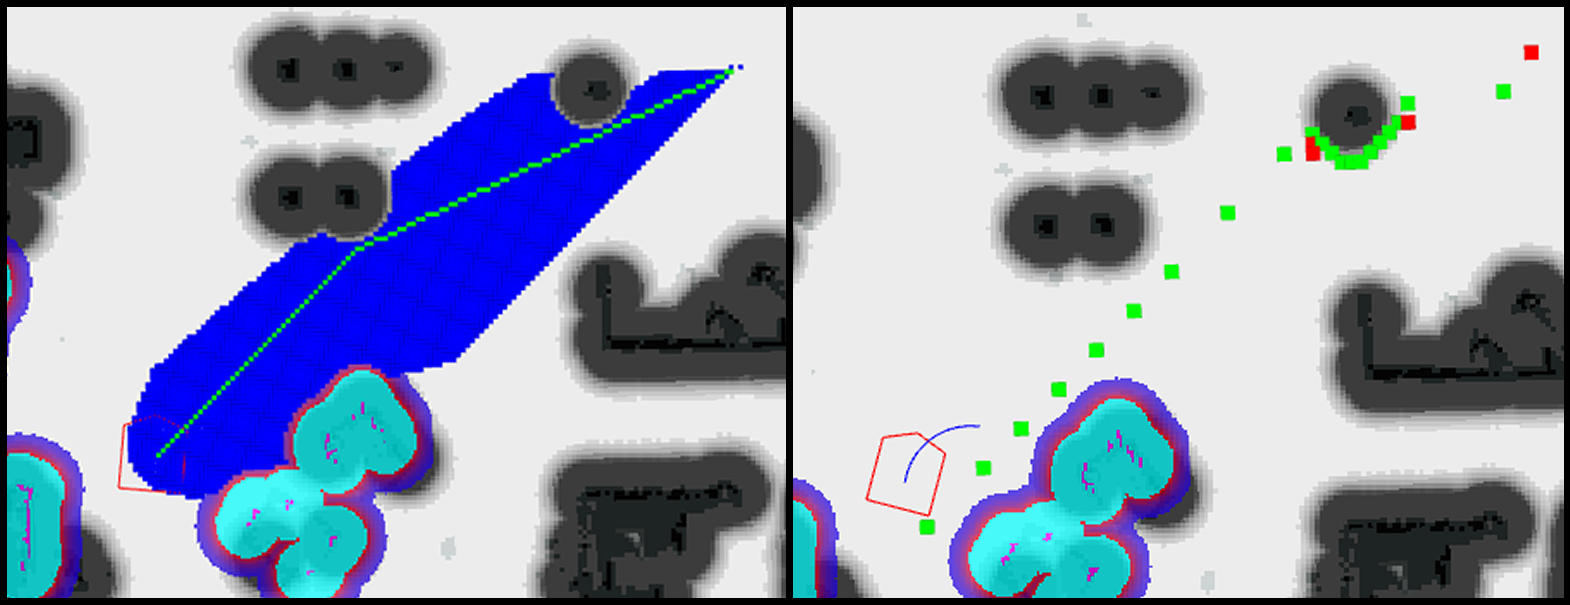
\includegraphics[scale=.26]{1_a}
  \caption{Ejecución de A* (izquierda) y Block A* (derecha).}
  \end{center}
\end{figure}

\begin{table}[H]
\begin{center}
 \begin{tabular}{|c|c|c|c|} 
 \hline
 \rule{0cm}{0.5cm}
 \textbf{Algoritmo} & \textbf{Tiempo (s)} & \textbf{Nodos expandidos} & \textbf{Distancia} \\
 \hline\hline
 \textbf{A*}       & 2.5 & 4001 & 7.98 \\ 
 \hline
 \textbf{Block A*} & 0 & 24 & 8.74 \\
 \hline
\end{tabular}
\caption{Resultados de la ejecución.}
\end{center}
\end{table}

Block A* ha reducido el número de nodos en un 99.4\% y aumentado la distancia en un 9.52\%.

\subsection{Expermiento 2}

Se han ejecutado los algoritmos para un camino de mediana distancia, desde la posición (46.66, 41.87) hasta la posición (30.07, 24.34).

En la Figura 1 se pueden ver los resultados de las distintas ejecuciones y en la Tabla 2 se recogen los datos.

\begin{figure}[H]
  \begin{center}
  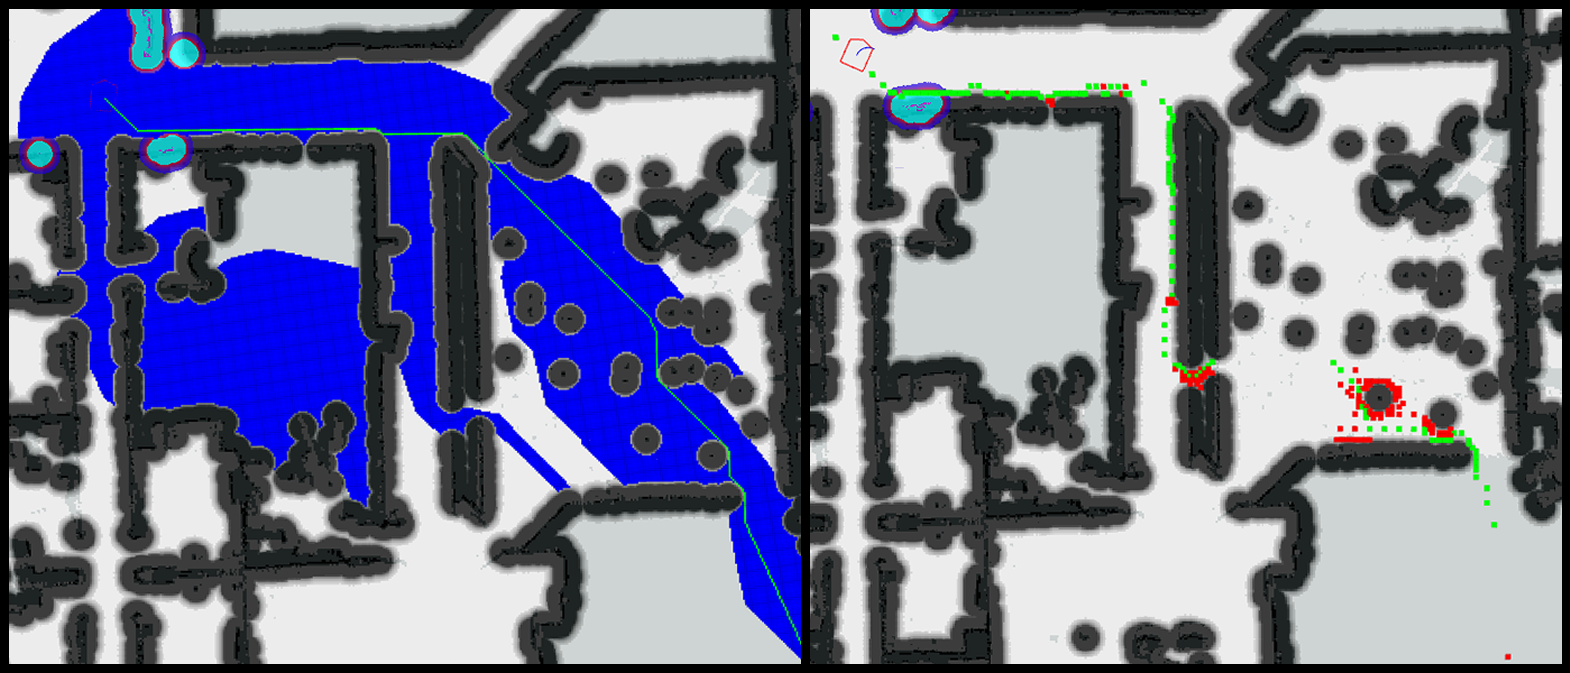
\includegraphics[scale=.26]{2_a}
  \caption{Ejecución de A* (izquierda) y Block A* (derecha).}
  \end{center}
\end{figure}

\begin{table}[H]
\begin{center}
 \begin{tabular}{|c|c|c|c|} 
 \hline
 \rule{0cm}{0.5cm}
 \textbf{Algoritmo} & \textbf{Tiempo (s)} & \textbf{Nodos expandidos} & \textbf{Distancia} \\
 \hline\hline
 \textbf{A*}       & 287 & 39277 & 28.25 \\ 
 \hline
 \textbf{Block A*} & 0 & 261 & 34.77 \\
 \hline
\end{tabular}
\caption{Resultados de la ejecución.}
\end{center}
\end{table}

Block A* ha reducido el número de nodos en un 99.34\% y aumentado la distancia en un 23.12\%.

\subsection{Expermiento 3}

Se han ejecutado los algoritmos para un camino de mediana distancia con muchos obstáculos, desde la posición (21.34, 40.07) hasta la posición (17.69, 11.29).

En la Figura 3 se pueden ver los resultados de las distintas ejecuciones y en la Tabla 3 se recogen los datos.

\begin{figure}[H]
  \begin{center}
  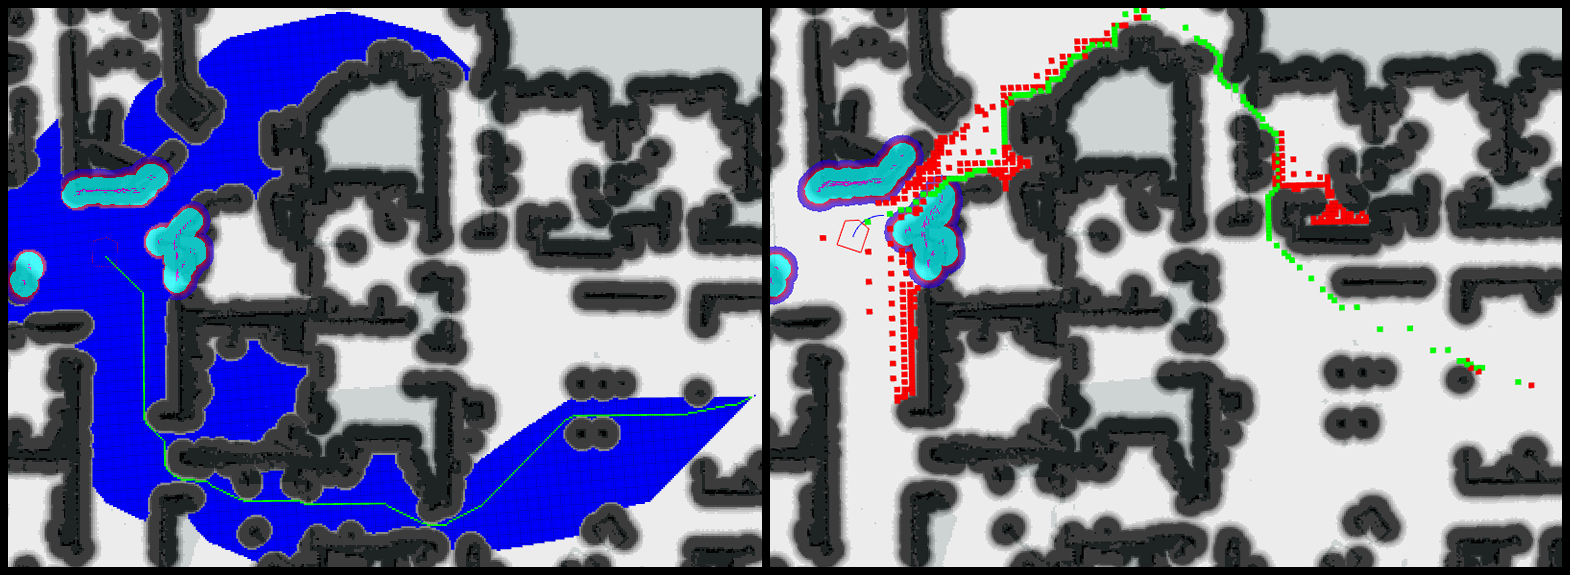
\includegraphics[scale=.26]{3_a}
  \caption{Ejecución de A* (izquierda) y Block A* (derecha).}
  \end{center}
\end{figure}

\begin{table}[H]
\begin{center}
 \begin{tabular}{|c|c|c|c|} 
 \hline
 \rule{0cm}{0.5cm}
 \textbf{Algoritmo} & \textbf{Tiempo (s)} & \textbf{Nodos expandidos} & \textbf{Distancia} \\
 \hline\hline
 \textbf{A*}       & 117.8 & 28149 & 24.68 \\ 
 \hline
 \textbf{Block A*} & 0 & 473 & 29.48 \\
 \hline
\end{tabular}
\caption{Resultados de la ejecución.}
\end{center}
\end{table}

Block A* ha reducido el número de nodos en un 98.32\% y aumentado la distancia en un 19.49\%.

\section{Conclusión}

Block A* por Niveles con las estructuras de datos utilizadas supera enormemente en tiempos de ejecución al algoritmo clásico debido además a la gran reducción de nodos, siendo su ejecución casi instantánea y ofreciendo por tanto una solución en tiempo real. De media se ha reducido el número de nodos a un 99.02\%.

A cambio de este beneficio, el camino generado es de mayor distancia, siendo este un camino subóptimo un 17.37\% más largo de media.

\section{Bibliografía}

\begin{thebibliography}{9}
\bibitem{autores} 
Peter Yap, Neil Burch, Robert C. Holte and Jonathan Schaeffer.
\textit{Any-Angle Path Planning for Computer Games}.
\end{thebibliography}

%----------------------------------------------------------------------------------------

\end{document}